\section{Satimo StarLab Anechoic Chamber}

\begin{aautop}
    The farfield measurements for this project will be carried out in a StarLab anechoic chamber by Satimo. In this section, the basic principles of doing measurements in this chamber will be described.
\end{aautop}

\begin{figure}[htbp]
    \centering
    \begin{subfigure}[t]{0.49\linewidth} 
        \centering
        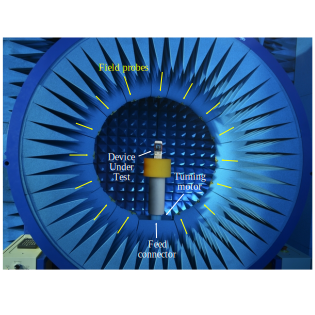
\includegraphics{img/analysis/satimo}
        \caption{Satimo StarLab. Modified from \cite{satimo}.}
        \label{fig:starlabchamber}
    \end{subfigure}
    \hfill
    \begin{subfigure}[t]{0.49\linewidth}
        \centering
        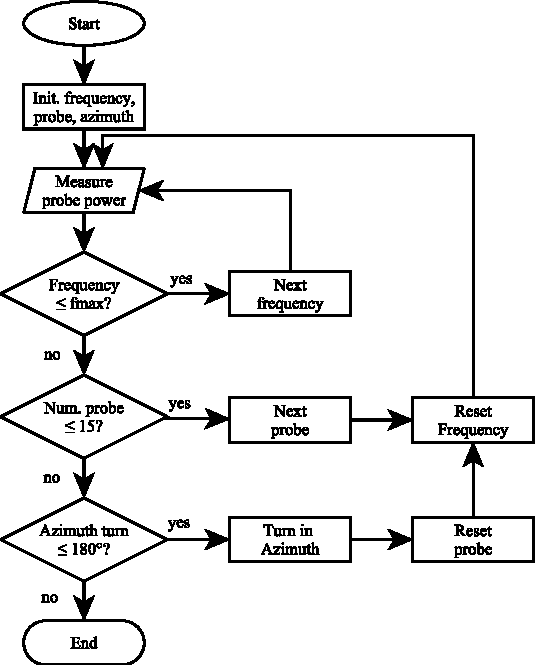
\includegraphics{img/analysis/satimoflow}
        \caption{Flow of a typical passive Satimo measurement.}
        \label{fig:satimoflow}
    \end{subfigure}
    \caption{Satimo StarLab passive measurement procedure.}
\end{figure}

The Satimo chamber is shown in Figure~\ref{fig:starlabchamber}. It consists of fifteen dual-polarized probes arranged in a circle with \ang{22.5} between each. The probes are located in a circle of absorbing cones and the whole machine is placed in a shielded room.

% Passive measurements: Power -> Antenna -> Probes
% What is measured?
The measurements used in this project are passive measurements. This means that the power is supplied from outside the chamber to the Device Under Test (DUT), which then radiates. The source is a user defined frequency sweep. For each frequency, the real and imaginary field at each probe for each polarization is sampled and recorded to a PC. After all frequencies for all probes have been recorded, the bed of the DUT turns, e.g.\ \ang{22.5}, and the procedure repeats. The flow is shown in Figure~\ref{fig:satimoflow}. The output is stored in a \texttt{trx} file in the order described by the flow chart. The post processing of the \texttt{trx} files is described thoroughly in Appendix~\ref{cha:postproc}.

% What we will use: Efficiency and correlation
% Calibration: Reference gain and efficiency
The measurements used for this report will mainly be used to compute the total efficiency of the DUT.
The efficiency can be computed by first calibrating the measurements by measuring a reference antenna with a known efficiency. The procedure for this is described in Section~\ref{sec:mimoant}.

%% Sources of error
The Satimo chamber is quite a complex system, and there are many sources of error. However, some of them are the same as with the VNA, which was described in Section~\ref{vna:errorSource}. Furthermore, there can be current flowing on the cable, bad connections, misaligned probes and inaccuracy in the motor rotations. 

\begin{aautail}
In this section, the Satimo StarLab chamber has been described. Based on this, the farfields can be measured of the antennas. By measuring reference antennas, the total efficiency can be computed. 
This section concludes the problem analysis, and the fundamental theorems and theories behind this project have been described. This leads to the final problem statement, which will briefly sum up the problem investigated throughout the rest of the report.
\end{aautail}
